\section{summary}
\begin{frame}
    \frame{\frametitle{Generative Adversarial Networks - Summary}}
	% \myheading{Module 23.5: Bringing it all together (the deep generative summary)}
\end{frame}

\begin{frame}
	\begin{overlayarea}{\textwidth}{\textheight}
	\begin{table}[]
	\def\arraystretch{1.5}%
\resizebox{0.8\textwidth}{!}{%
\begin{tabular}{c|cccc}
             & RBMs                  & VAEs                  & AR models     & GANs        \\
%\hline
%\hline

Abstraction  & Yes                   & Yes                   & No            & No          \\
\onslide<2->{Generation}   & \onslide<2->{Yes                   & Yes                   & Yes           & Yes}         \\
\onslide<3->{Compute P(X)} & \onslide<3->{Intractable           & Intractable           & Tractable     & No }         \\
\onslide<4->{Sampling     }& \onslide<4->{MCMC                  & Fast                  & Slow          & Fast }       \\
\onslide<5->{Type of GM  } & \onslide<5->{Undirected            & Directed              & Directed      & Directed}    \\
\onslide<6->{Loss       }  & \onslide<6->{KL-divergence         & KL-divergence         & KL-divergence & JSD }        \\
\onslide<7->{Assumptions}  & \onslide<7->{X independent given z & X independent given z & None          & N.A. }       \\
\onslide<8->{Samples}      & \onslide<8->{Bad                   & Ok                    & Good          & Good (best)} \\
\end{tabular}}
\caption{Comparison of Generative Models}
\label{my-label}
\end{table}
\only<9->{
\small
\textit{
Recent works look at combining these methods: e.g. Adversarial Autoencoders (Makhzani 2015), PixelVAE (Gulrajani 2016) and PixelGAN Autoencoders (Makhzani 2017)}}

	\end{overlayarea}
\end{frame}

\begin{frame}
	\begin{figure}[h!]
		%\vspace*{-1mm}
		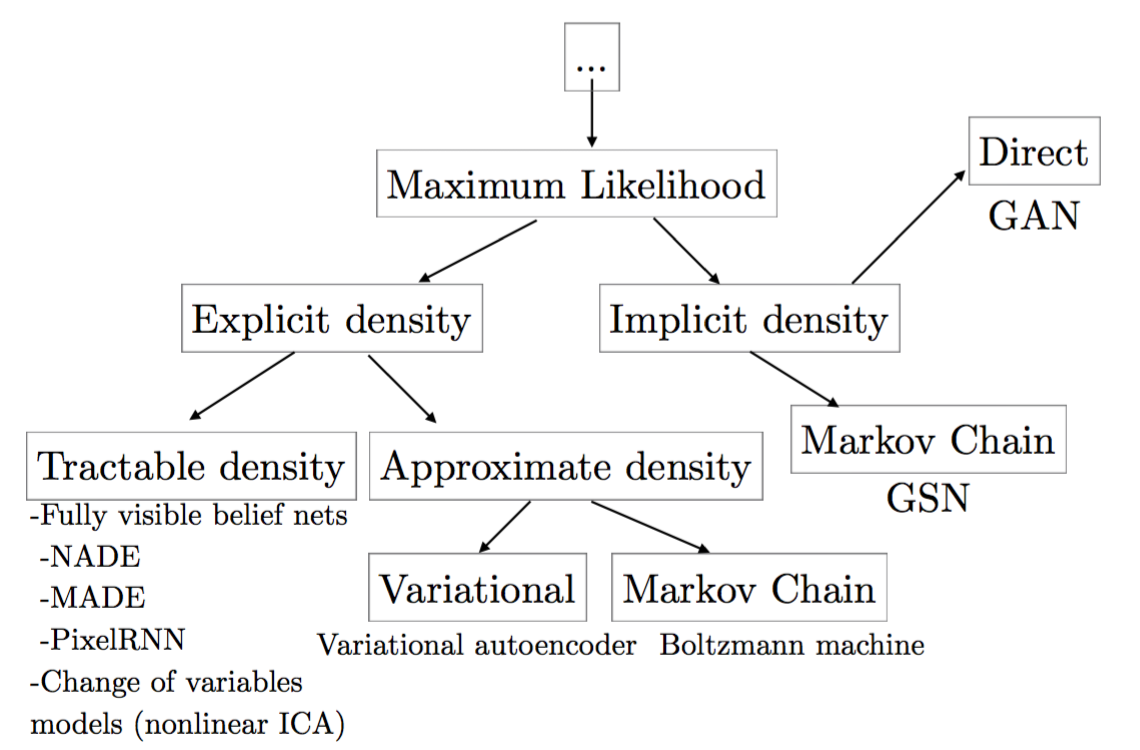
\includegraphics[scale=0.40]{images/Taxonomy.png}
	\end{figure}
	\textbf{Source:} Ian Goodfellow, NIPS 2016 Tutorial: Generative Adversarial Networks
\end{frame}

